\documentclass[a4paper,twoside]{ctexart}
\usepackage{geometry}
\geometry{margin=1cm,vmargin={0pt,1cm}}
\setlength{\topmargin}{-2cm}
\setlength{\paperheight}{23cm}
\setlength{\paperwidth}{18cm}
\setlength{\textheight}{19.6cm}
\setlength{\textwidth}{15cm}
\usepackage{makecell}
\usepackage{fancyhdr}
\usepackage{siunitx}
\usepackage{amssymb}
\usepackage{indentfirst}
\setlength{\parindent}{0.5em}

\pagenumbering{arabic}

% useful packages.
\usepackage{multirow}
\usepackage{caption}
\usepackage{mathrsfs}
\usepackage{amsfonts}
\usepackage{amsmath}
\usepackage{amsthm}
\usepackage{enumerate}
\usepackage{xcolor,graphicx,float,subfigure}
\usepackage{epstopdf}
\usepackage{multicol}
\usepackage{fancyhdr}
\usepackage{layout}
\usepackage{listings}
\lstset{language=Matlab}
\lstset{breaklines}
\lstset{extendedchars=false}
\usepackage[colorlinks,linkcolor=blue]{hyperref}
\usepackage{xcolor}
\usepackage{cite}
\usepackage[numbers,sort&compress]{natbib} 
\setcitestyle{open={},close={}}
%\usepackage{natbibspacing}
%\renewcommand{\refname}{}
\usepackage{anyfontsize}
%\usepackage[ruled]{algorithm2e}
\usepackage{algorithm}
\usepackage{algorithmicx}
\usepackage{algpseudocode}
\renewcommand{\algorithmicrequire}{\textbf{Input:}}  % Use Input in the format of Algorithm
\renewcommand{\algorithmicensure}{\textbf{Side effect:}} % Use Output in the format of Algorithm


\usepackage{bm}



% some common command
\newcommand{\dif}{\mathrm{d}}
\newcommand{\avg}[1]{\left\langle #1 \right\rangle}
\newcommand{\pdfrac}[2]{\frac{\partial #1}{\partial #2}}
\newcommand{\op}{\odot}
\newcommand{\Eabs}{E_{\mathrm{abs}}}
\newcommand{\Erel}{E_{\mathrm{rel}}}
\newcommand{\Ediv}{\mathrm{div}}%\div是除号
\newcommand{\lrq}[1]{\left( #1 \right)}
\newcommand{\avint}[1]{\frac{1}{\left|#1\right|}\int_{#1}}

\newcommand{\upcite}[1]{\textsuperscript{\textsuperscript{\cite{#1}}}}


\makeatletter
\newcommand\sixteen{\@setfontsize\sixteen{17pt}{6}}
\renewcommand{\maketitle}{\bgroup\setlength{\parindent}{0pt}
\begin{flushleft}
\sixteen\bfseries \@title
\medskip
\end{flushleft}
\textit{\@author}
\egroup}
\makeatother

\CTEXsetup[format={\Large\bfseries}]{section}

\title{MARS2D 测试文档}


\begin{document}
\maketitle
\vspace{-3em}
\section{LUD分解}
LUD分解是用来求解系数矩阵为循环三对角矩阵的线性方程组的:
\begin{equation}
  \bm{A}\bm{x}=
  \begin{bmatrix}
    b_1&c_1   &      &a_1\\
    a_2&\ddots&\ddots&\\
       &\ddots&\ddots&c_{n-1}\\
    c_n&      &a_n   &b_n
  \end{bmatrix}\bm{x}=\bm{b}.
\end{equation}
在程序中主要用于循环三次样条插值中。

首先对$\bm{A}$进行第一次分解:
\begin{equation}
  \bm{A}=\begin{bmatrix}
    b_1&c_1   &      &a_1\\
    a_2&\ddots&\ddots&\\
       &\ddots&\ddots&c_{n-1}\\
    c_n&      &a_n   &b_n
  \end{bmatrix}=
  \begin{bmatrix}
    p_1&&&&\\
    a_2&p_2   &&&\\
       &\ddots&\ddots&&\\
       &      &\ddots&\ddots&\\
       &      &      &a_n   &p_n
  \end{bmatrix}
  \begin{bmatrix}
    1&q_1   &      &       &r_1\\
     &\ddots&\ddots&       &\vdots\\
     &      &1     &q_{n-2}&r_{n-2}\\
     &      &      &1      &r_{n-1}\\
    s&      &      &       &1
  \end{bmatrix}=\bm{L}\tilde{\bm{U}},
\end{equation}
其中
\begin{equation}
  \left\{
  \begin{array}{l}
    p_1=b_1,q_1=c_1/p_1,r_1=a_1/p_1;\\
    p_i=b_i-a_i q_{i-1},q_i=c_i/p_i,r_i=-a_i r_{i-1}/p_i,i=2,\cdots,n-2;\\
    p_{n-1}=b_{n-1}-a_{n-1}q_{n-2},r_{n-1}=(c_{n-1}-a_{n-1}r_{n-2})/p_{n-1};\\
    p_n=b_n-a_n r_{n-1},s=c_n/p_n.
  \end{array}
  \right.
\end{equation}

再对$\tilde{\bm{U}}$进行分解:
\begin{equation}
  \tilde{\bm{U}}=\begin{bmatrix}
    1&q_1   &      &       &r_1\\
     &\ddots&\ddots&       &\vdots\\
     &      &1     &q_{n-2}&r_{n-2}\\
     &      &      &1      &r_{n-1}\\
    s&      &      &       &1
  \end{bmatrix}=
  \begin{bmatrix}
    1&q_1&&&\\
     &\ddots&\ddots&&\\
     &      &1     &q_{n-2}&\\
     &      &      &1      &0\\
     &      &      &       &1
  \end{bmatrix}
  \begin{bmatrix}
    1&      & & &t_1\\
     &\ddots& & &\vdots\\
     &      &1& &t_{n-2}\\
     &      & &1&t_{n-1}\\
    s&      & & &1
  \end{bmatrix}=\bm{U}\bm{D},
\end{equation}
其中
\begin{equation}
  \left\{
    \begin{array}{l}
      t_{n-1}=r_{n-1};\\
      t_i=r_i-q_i t_{i+1},i=n-2,n-3,\cdots,1.
    \end{array}
  \right.
\end{equation}

之后分别求解$\bm{L}\bm{z}=\bm{b}$,$\bm{U}\bm{y}=\bm{z}$,$\bm{D}\bm{x}=\bm{y}$即可,这几个线性方程组都很容易求解。整体时间复杂度为$\mathrm{O}(n)$,$n$为系数矩阵的阶数。

\section{一种加减点方法:IMV}
这里介绍一下谭焱师兄提出来的一种加减点方法。

\texttt{List}在我们的程序中的缺点表现在建立临时变量慢,优点在于加减点是$\mathrm{O}(1)$时间复杂度的,所以我们要进行改进就要找到一种方法,既能避免建立\texttt{List}临时变量,又同时保持加减点的时间复杂度是$\mathrm{O}(1)$的。由于我们是基于\texttt{Vector}实现的,所以这种方法我们暂且叫它IMV(Improved Vector)方法。
\vspace{-1em}
\subsection{容器}
使用\texttt{Vector}来存储示踪点列,这样在每一个时间步中就是创建一个\texttt{Vector}临时变量而不是\texttt{List}。
\vspace{-1em}
\subsection{减点算法}
\begin{algorithm}[h]
  \begin{algorithmic}[1]
	\Require
    \texttt{Vector<Point> \&pts; Vector<bool> tag; tag的第一个和最后一个元素一定为false;}
  \Ensure
	  \texttt{pts中tag[i]为true的对应点pts[i]将被删除;}
  \State \texttt{第一个点一定不会被删,从第二个点开始;}
  \State \texttt{int count = 1;}
	\For{\texttt{(int i = 1; i<pts.size(); i++)}}
	 	\If{\texttt{tag[i]==false}}
      \If{\texttt{count!=i}}
        \State \texttt{pts[count] = pts[i];}
      \EndIf
      \State \texttt{count++;}
    \EndIf
  \EndFor
  \State \texttt{pts.resize(count);}
  \end{algorithmic}
 	\caption{removeMarkers}
 	\label{alg:remove} 
\end{algorithm} 

如算法\ref{alg:remove}所示。在这里我们在\texttt{pts}原址进行修改,因为减点后的示踪点列不会比原点列更长。我们用后面要保留的点覆盖掉前面要被删除的点的内存,最后\texttt{resize}一下就可以了。对于每个留下来的示踪点至多调用了一次拷贝构造函数,而对于删除的节点则什么都不需要做。
\vspace{-1em}
\subsection{加点算法}
\begin{algorithm}[h]
  \begin{algorithmic}[1]
    \Require
      \texttt{Vector<Point> \&pts; Real lowBound;}
	  \Ensure
      \texttt{在pts中距离过长的相邻点间加点;}
    \State \texttt{Vector<Point> res(2 * pts.size());}
    \State \texttt{res[0] = pts[0];}
    \State \texttt{int count = 1;}
	  \For{\texttt{(int i = 0; i<pts.size()-1; i++)}}
	 	  \If{\texttt{norm(pts[i+1]-pts[i])>lowBound}}
       \State \texttt{localpts = 需要添加的点列;}
        \For{\texttt{auto $\&$lpt : localpts}}
          \State \texttt{res[count] = lpt;}
          \State \texttt{检查res容量是否已满,满则扩容;}
          \State \texttt{count++;}
        \EndFor
      \EndIf
      \State \texttt{res[count] = pts[i+1];}
      \State \texttt{检查res容量是否已满,满则扩容;}
      \State \texttt{count++;}
    \EndFor
    \State \texttt{res.resize(count);}
    \State \texttt{pts = res;}
  \end{algorithmic}
 	\caption{addMarkers}
 	\label{alg:split} 
\end{algorithm}

如算法\ref{alg:split}所示。在这里我们首先建立了一个\texttt{Vector}临时变量,并且分配了比较多的内存,用来存储加点后的示踪点列。对于每个示踪点我们调用了一次拷贝构造函数,并做了一次是否即将越界的判断。而对于每个新加入的点,插入的时间复杂度是$\mathrm{O}(1)$的。

这样我们就实现了既不建立\texttt{List}临时变量,对每个点的插入和删除的时间复杂度又控制在了$\mathrm{O}(1)$内。代价是不论是否真的需要加点,在\texttt{split}函数中都要创建临时的\texttt{Vector}变量并调用拷贝构造。

\section{测试结果}
以下两个测试都是针对 Cubic MARS 方法的即殷集边界是用三次样条曲线表示的。测试中首先在某一个圆上均匀取点,之后由这些点生成的三次样条曲线作为初值。$h_L$取值为两个初值点间弧长的$2$倍。在CPU时间这部分,我们对三种方法进行了测试,第一种是用\texttt{Vector}容器的,第二种是用\texttt{List}容器的,第三种使用上一节中的IMV的,结果取10次测试的平均值。
\subsection{Vortex shear of a circular disk}
速度场如下:
\begin{equation}
  \left\{
  \begin{array}{l}
    u_x=\cos\left(\pi \dfrac{t}{T}\right)\sin^2(\pi x)\sin(2\pi y);\\
    u_y=-\cos\left(\pi \dfrac{t}{T}\right)\sin(2\pi x)\sin^2(\pi y).
  \end{array}
  \right.
\end{equation}  

测试所用参数如表\ref{tab:vortex1}所示。
\begin{table}[htbp]
    \centering\begin{tabular}{c|c}
        \hline
        参数&值\\
        \hline
        周期&$T=8$\\
        中心点&$C=(0.5,0.75)$\\
        半径&$R=0.15$\\
        $r_{\mathrm{tiny}}$&$r_{\mathrm{tiny}}=0.01$\\
        初值点数&$n=64,128,256,512,1024$\\
        时间步长&$k=4\mathrm{e}-2,2\mathrm{e}-2,1\mathrm{e}-2,5\mathrm{e}-3,2.5\mathrm{e}-3$\\
        \hline
    \end{tabular}
    \caption{Vortex shear: 参数表}
    \label{tab:vortex1}
\end{table}

测试结果如表\ref{tab:vortex2}所示,所用误差范数$\|\mathrm{E}\|_1$是用计算出的三次样条曲线和用准确解正圆上的点生成的三次样条曲线求内部区域间近似异或面积得出的。发现可以测得四阶以上的收敛阶。

\begin{table}[htbp]
    \centering\begin{tabular}{c|ccccccccc}
        \hline
        $h_L=4\pi/n$&$n=64$&ratio&128&ratio&256&ratio&512&ratio&1024\\
        \hline
        $\|\mathrm{E}\|_1$&4.80e-5&4.25&2.52e-6&4.96&8.08e-8&7.41&4.77e-10&4.09&2.80e-11\\
        \hline
        Vector: CPU time(s)&2.91e-1&1.87&1.06&1.95&4.11&1.99&1.64e+1&2.02&6.63e+1\\
        \hline
        List: CPU time(s)&3.13e-1&1.87&1.15&1.96&4.45&1.98&1.76e+1&2.01&7.11e+1\\
        \hline
        IMV: CPU time(s)&2.83e-1&1.92&1.07&1.95&4.14&1.99&1.64e+1&2.02&6.65e+1\\
        \hline
    \end{tabular}
    \caption{Vortex shear: 误差、收敛阶及运行时间对比}
    \label{tab:vortex2}
\end{table}

中间步的计算结果图如图\ref{fig:vortex}所示。

\begin{figure}[H]
	\centering  %图片全局居中
	\subfigure[$t=0$]{
		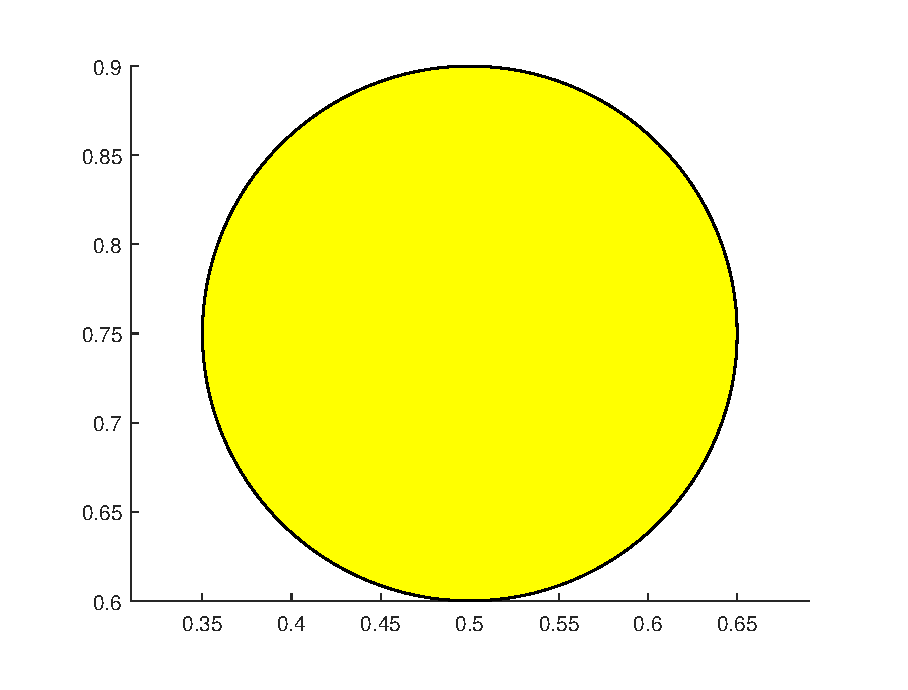
\includegraphics[width=0.3\linewidth]{vortex0T.eps}
    }
	\subfigure[$t=\dfrac{1}{8}T$]{
		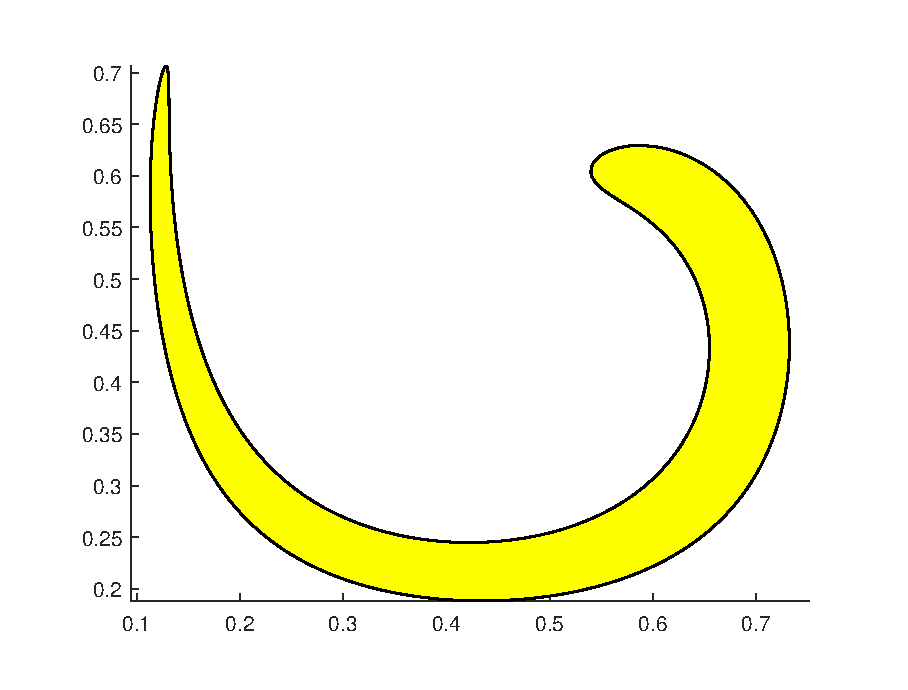
\includegraphics[width=0.3\linewidth]{vortex1_8T.eps}
    }
    \subfigure[$t=\dfrac{1}{4}T$]{
        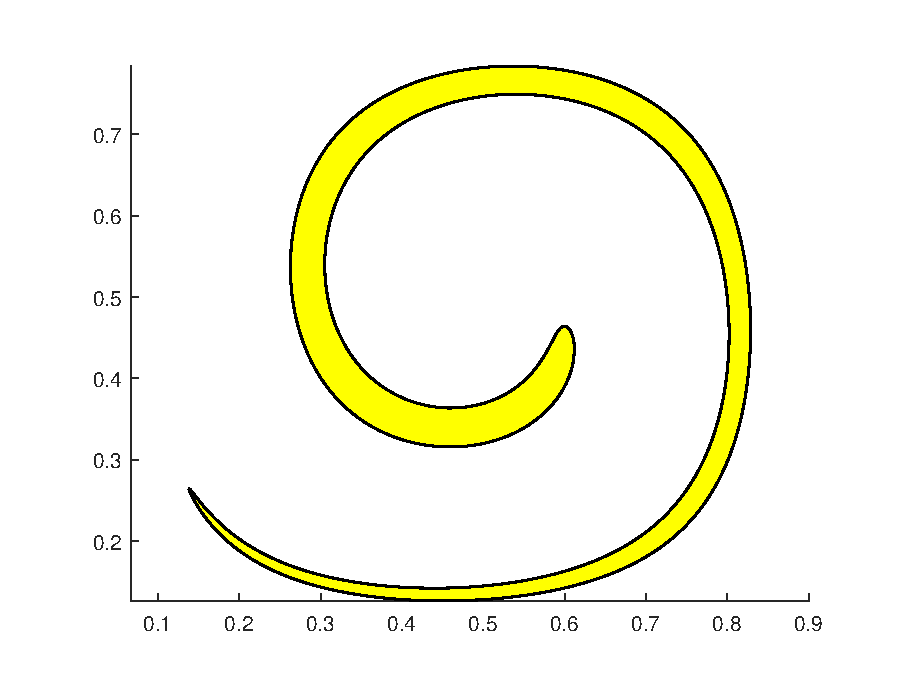
\includegraphics[width=0.3\linewidth]{vortex2_8T.eps}
    }\\
    \subfigure[$t=\dfrac{3}{8}T$]{
		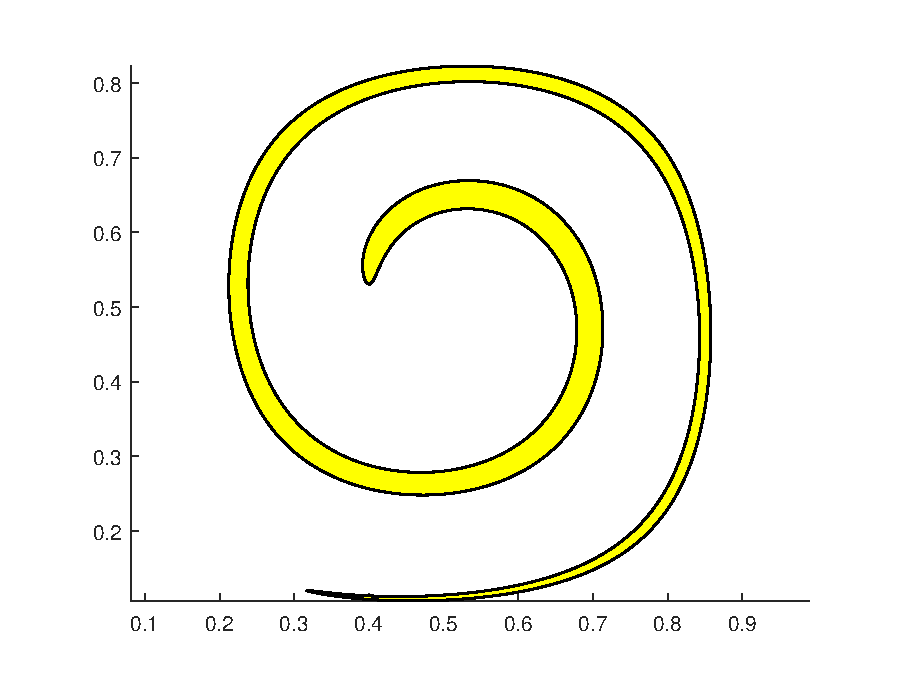
\includegraphics[width=0.3\linewidth]{vortex3_8T.eps}
    }
	\subfigure[$t=\dfrac{1}{2}T$]{
		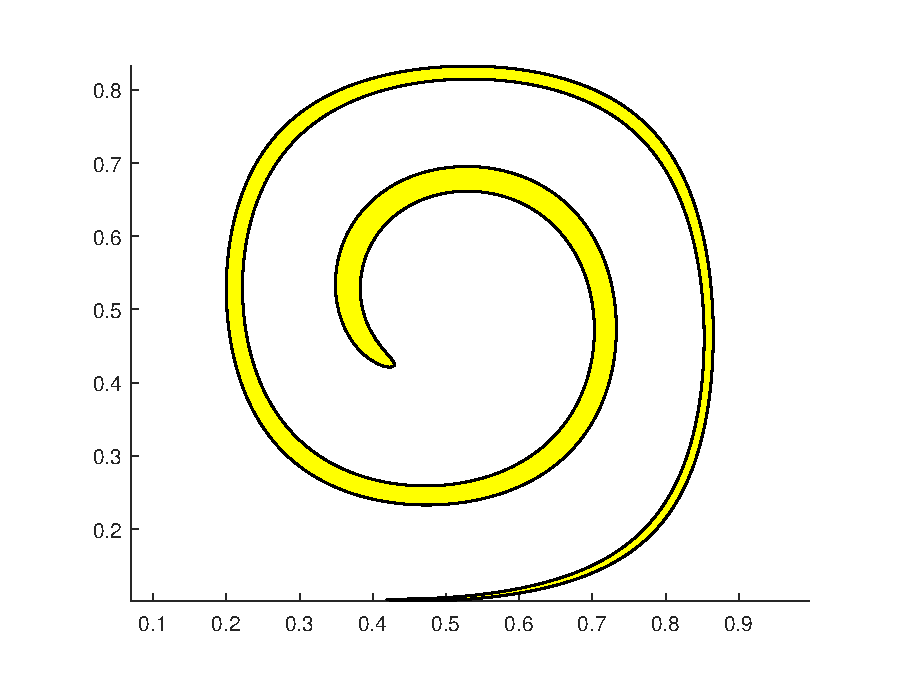
\includegraphics[width=0.3\linewidth]{vortex4_8T.eps}
    }
    \subfigure[$t=\dfrac{5}{8}T$]{
        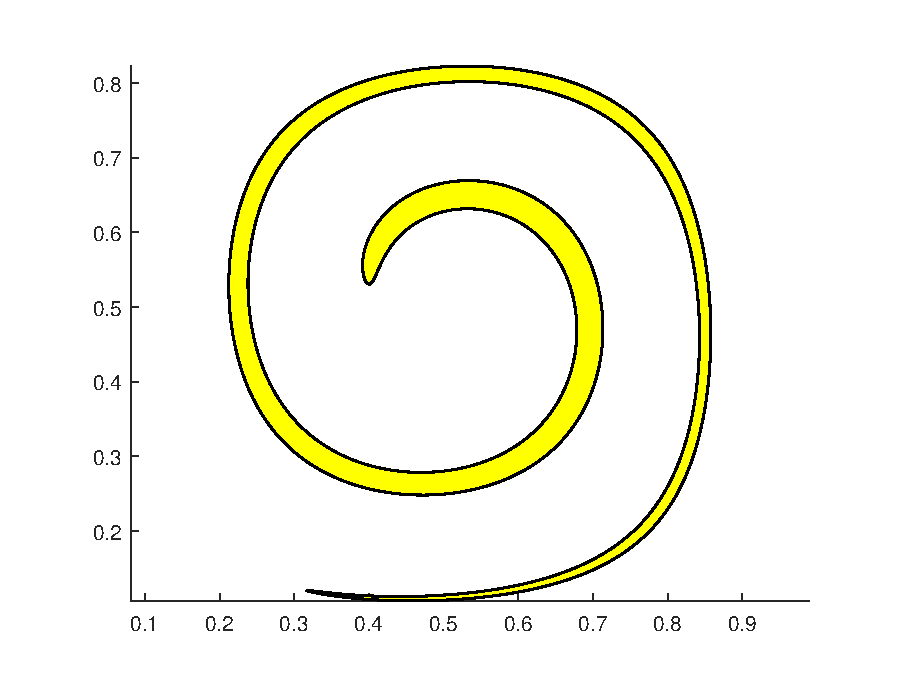
\includegraphics[width=0.3\linewidth]{vortex5_8T.eps}
    }\\
    \subfigure[$t=\dfrac{3}{4}T$]{
		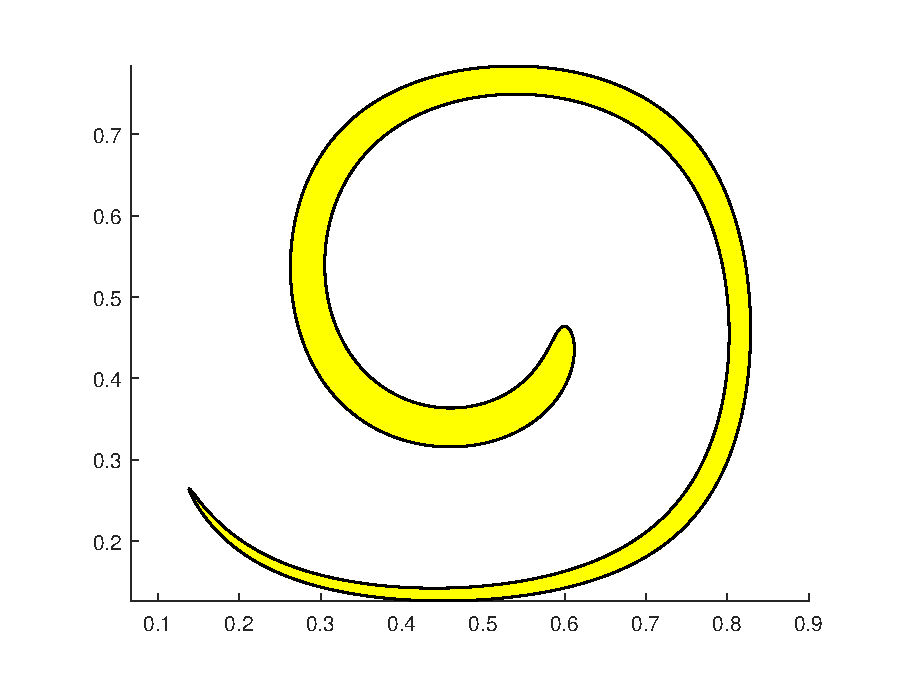
\includegraphics[width=0.3\linewidth]{vortex6_8T.eps}
    }
	\subfigure[$t=\dfrac{7}{8}T$]{
		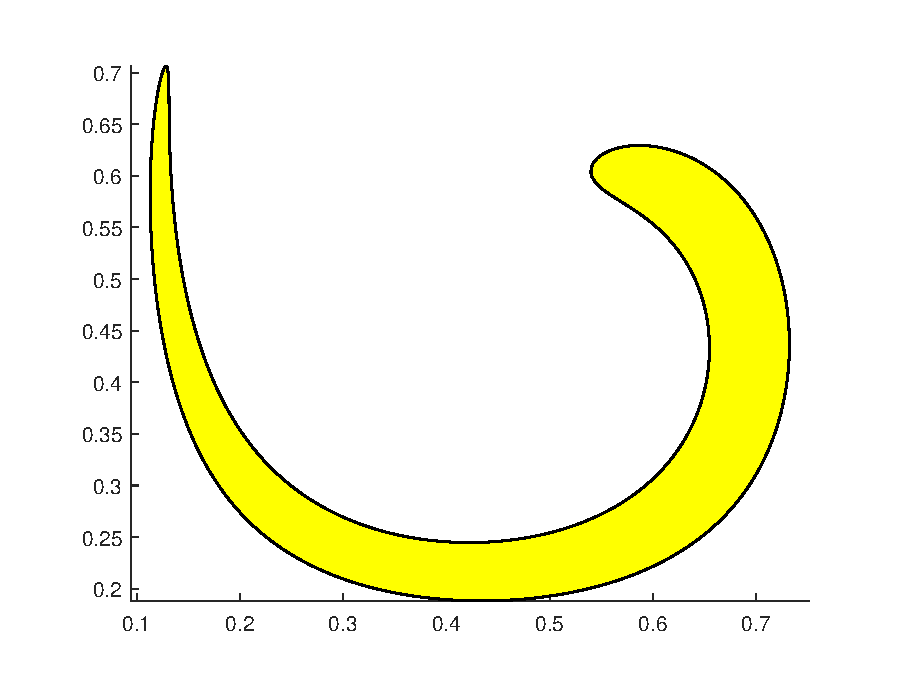
\includegraphics[width=0.3\linewidth]{vortex7_8T.eps}
    }
    \subfigure[$t=T$]{
        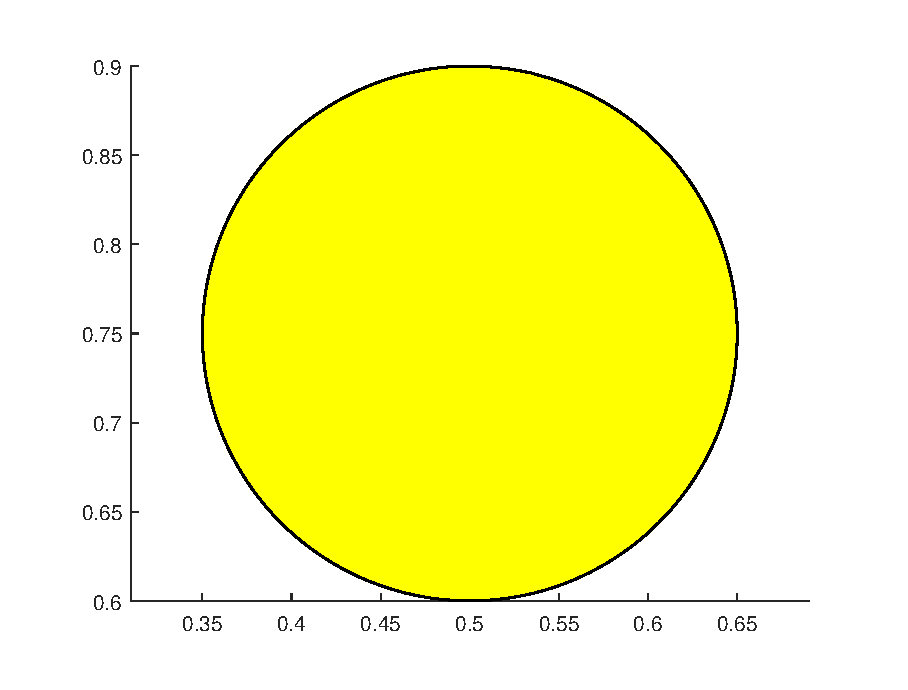
\includegraphics[width=0.3\linewidth]{vortex1T.eps}
    }
    \caption{Vortex shear: 中间步计算结果图,所用参数为 $n=128$,$k=2\mathrm{e}-2$,$r_\mathrm{tiny}=0.01$。}
    \label{fig:vortex}
\end{figure}

\subsection{Deformation of a circular disk}

速度场如下:
\begin{equation}
  \left\{
    \begin{array}{l}
      u_x=\cos\left(\pi \dfrac{t}{T}\right)\sin(n\pi(x+0.5))\sin(n\pi(y+0.5));\\
      u_y=\cos\left(\pi \dfrac{t}{T}\right)\cos(n\pi(x+0.5))\cos(n\pi(y+0.5));\\
      n=4.
    \end{array}
  \right.
\end{equation}

测试所用参数如表\ref{tab:deformation1}所示。这里我调整了一下测例,因为在这一次的测试中我发现$n=128$,$k=4\mathrm{e}-2$时计算出来的结果无法正确的逼近准确解正圆,所以将时间步长缩短了一半,发现所有计算解都可以很好的逼近准确解正圆。
\begin{table}[htbp]
    \centering\begin{tabular}{c|c}
        \hline
        参数&值\\
        \hline
        周期&$T=2$\\
        中心点&$C=(0.5,0.5)$\\
        半径&$R=0.15$\\
        $r_{\mathrm{tiny}}$&$r_{\mathrm{tiny}}=0.01$\\
        初值点数&$n=128,256,512,1024,2048$\\
        时间步长&$k=2\mathrm{e}-2,1\mathrm{e}-2,5\mathrm{e}-3,2.5\mathrm{e}-3,1.25\mathrm{e}-3$\\
        \hline
    \end{tabular}
    \caption{Deformation: 参数表}
    \label{tab:deformation1}
\end{table}

测试结果如表\ref{tab:deformation2}所示,所用误差范数$\|\mathrm{E}\|_1$是用计算出的三次样条曲线和用准确解正圆上的点生成的三次样条曲线求内部区域间近似异或面积得出的。发现可以测得四阶以上的收敛阶。

\begin{table}[htbp]
    \centering\begin{tabular}{c|ccccccccc}
        \hline
        $h_L=4\pi/n$&$n=128$&ratio&256&ratio&512&ratio&1024&ratio&2048\\
        \hline
        $\|\mathrm{E}\|_1$&2.43e-5&3.67&1.91e-6&5.20&5.19e-8&6.56&5.50e-10&4.12&3.07e-11\\
        \hline
        Vector: CPU time(s)&3.01e-1&1.99&1.19&2.01&4.81&2.00&1.93e+1&1.84&6.92e+1\\
        \hline
        List: CPU time(s)&3.26e-1&1.97&1.28&2.01&5.13&1.99&2.04e+1&1.84&7.29e+1\\
        \hline
        IMV: CPU time(s)&3.04e-1&1.97&1.20&2.01&4.81&2.00&1.92e+1&1.84&6.90e+1\\
        \hline
    \end{tabular}
    \caption{Deformation: 误差、收敛阶及运行时间对比}
    \label{tab:deformation2}
\end{table}

中间步的计算结果图如图\ref{fig:deformation}所示。
\begin{figure}[H]
	\centering  %图片全局居中
	\subfigure[$t=0$]{
		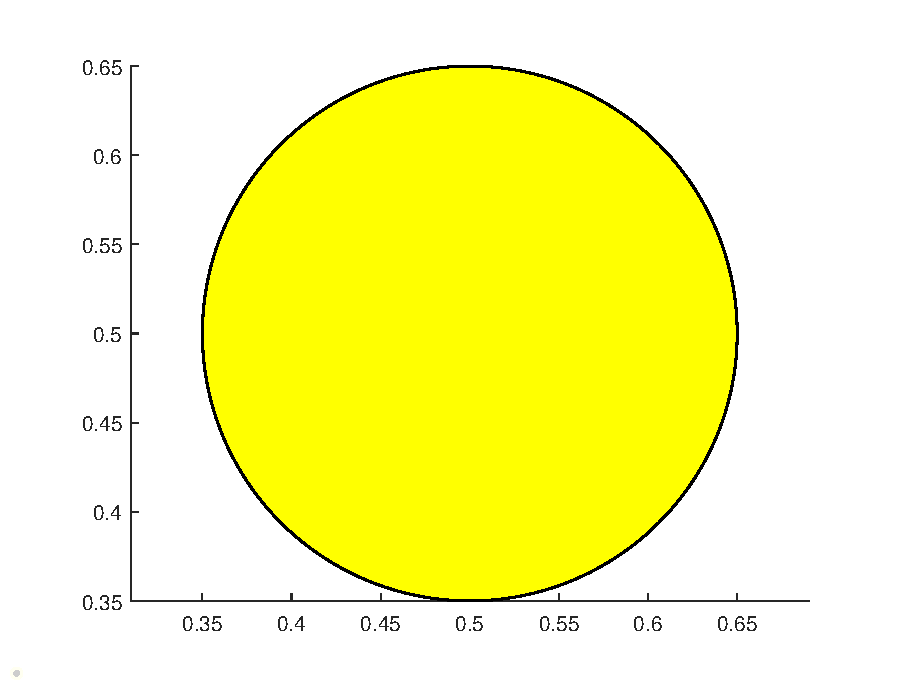
\includegraphics[width=0.3\linewidth]{deformation0T.eps}
    }
	\subfigure[$t=\dfrac{1}{8}T$]{
		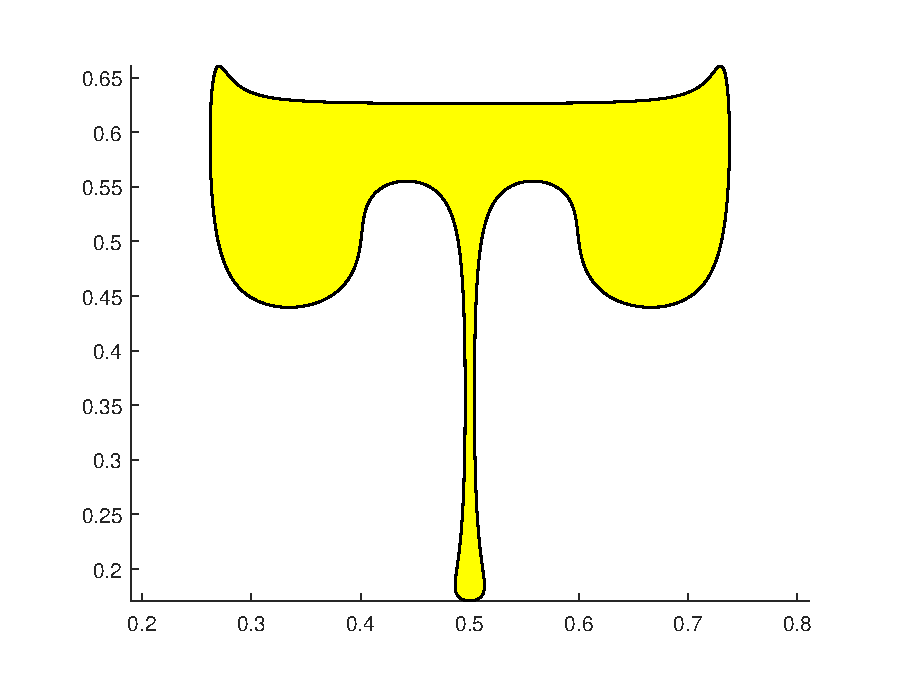
\includegraphics[width=0.3\linewidth]{deformation1_8T.eps}
    }
    \subfigure[$t=\dfrac{1}{4}T$]{
        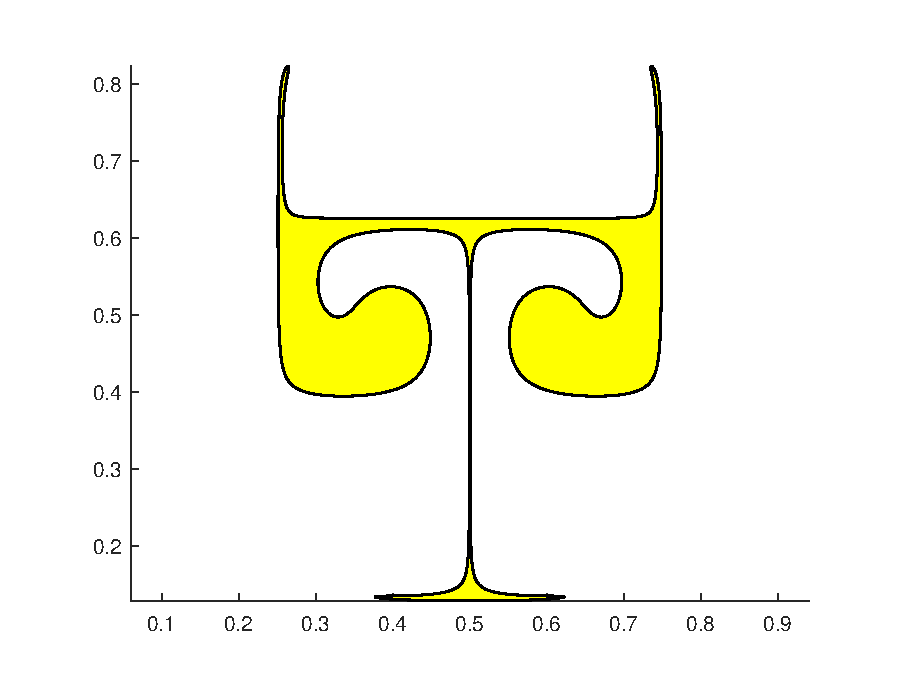
\includegraphics[width=0.3\linewidth]{deformation2_8T.eps}
    }\\
    \subfigure[$t=\dfrac{3}{8}T$]{
		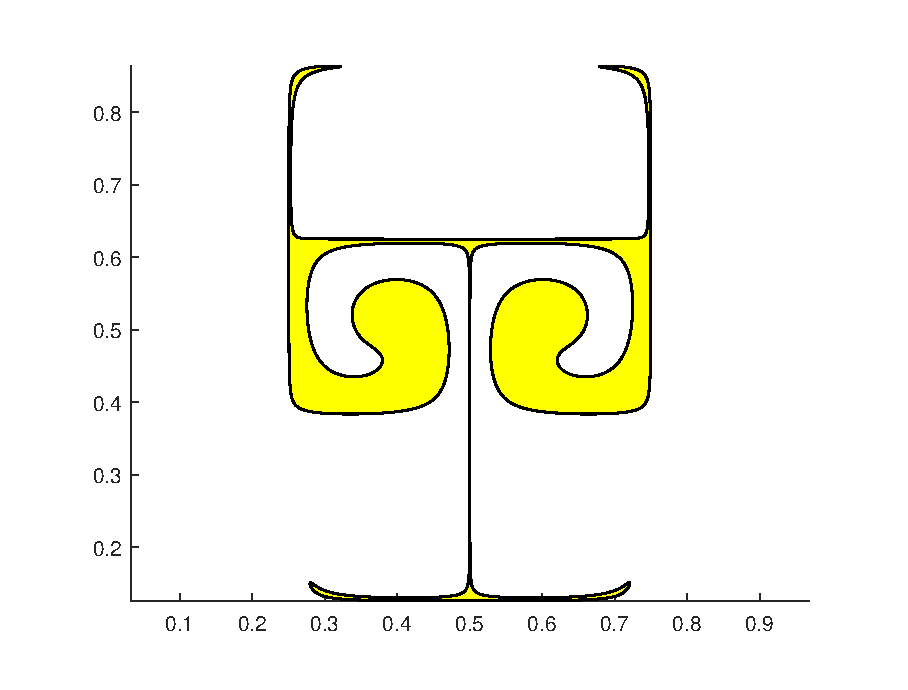
\includegraphics[width=0.3\linewidth]{deformation3_8T.eps}
    }
	\subfigure[$t=\dfrac{1}{2}T$]{
		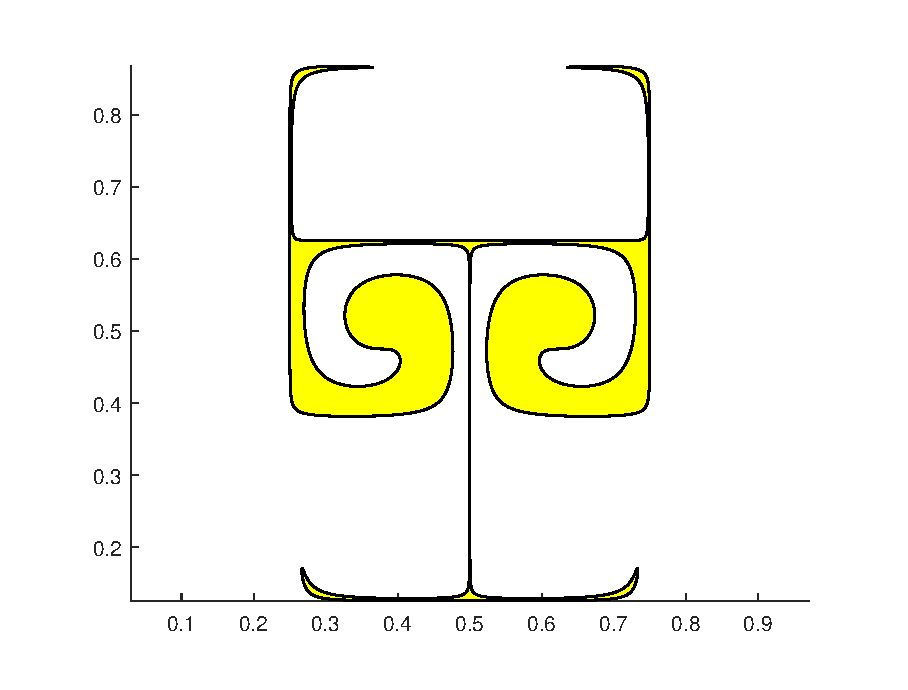
\includegraphics[width=0.3\linewidth]{deformation4_8T.eps}
    }
    \subfigure[$t=\dfrac{5}{8}T$]{
        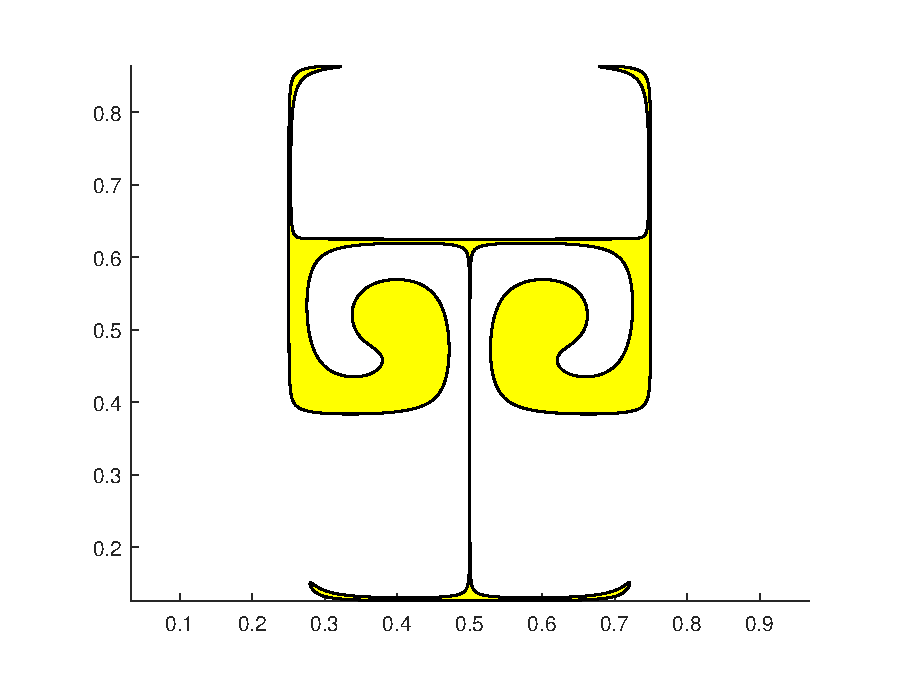
\includegraphics[width=0.3\linewidth]{deformation5_8T.eps}
    }\\
    \subfigure[$t=\dfrac{3}{4}T$]{
		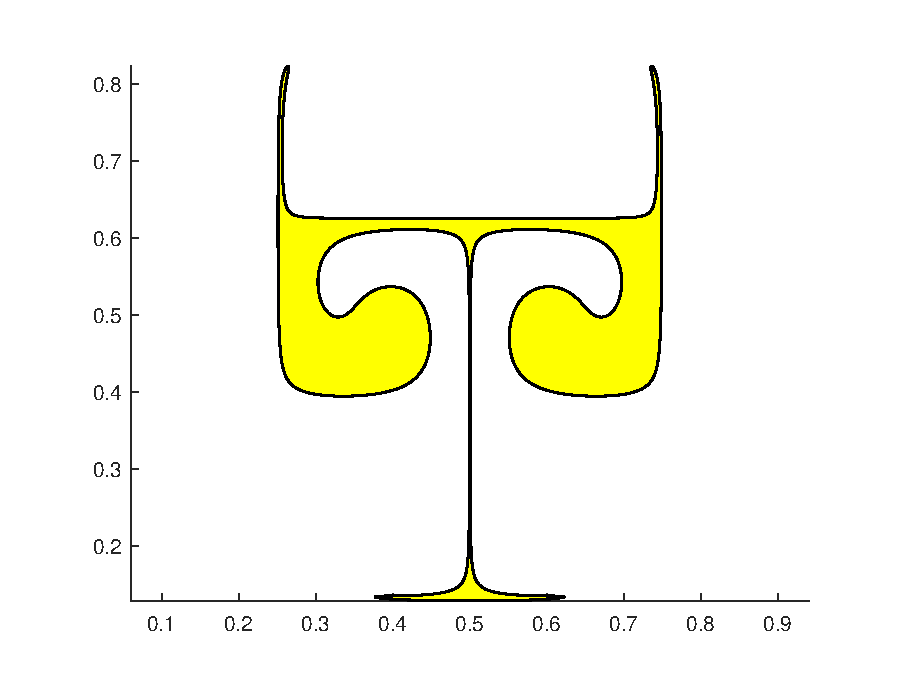
\includegraphics[width=0.3\linewidth]{deformation6_8T.eps}
    }
	\subfigure[$t=\dfrac{7}{8}T$]{
		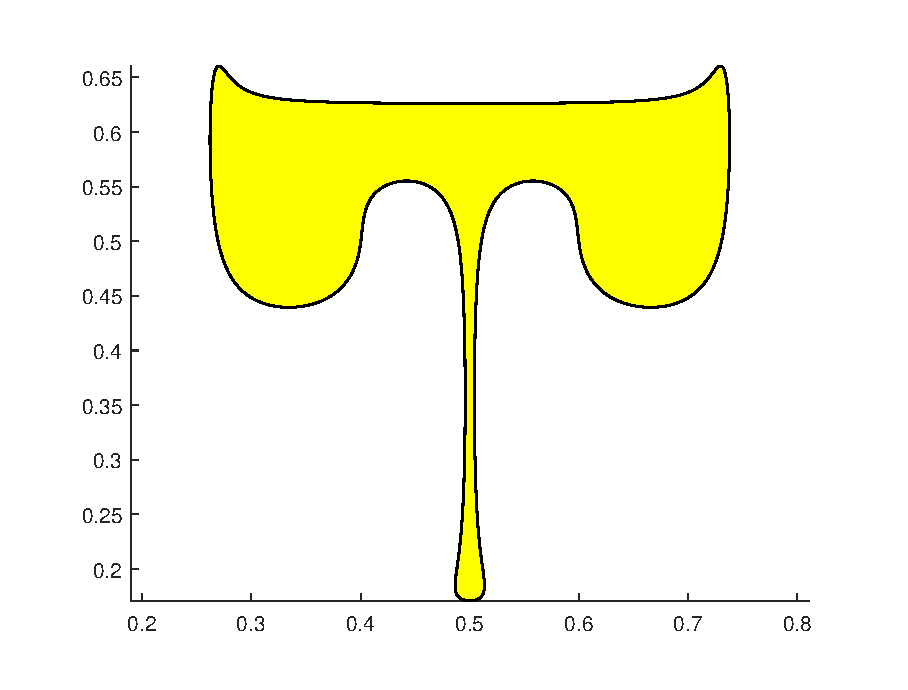
\includegraphics[width=0.3\linewidth]{deformation7_8T.eps}
    }
    \subfigure[$t=T$]{
        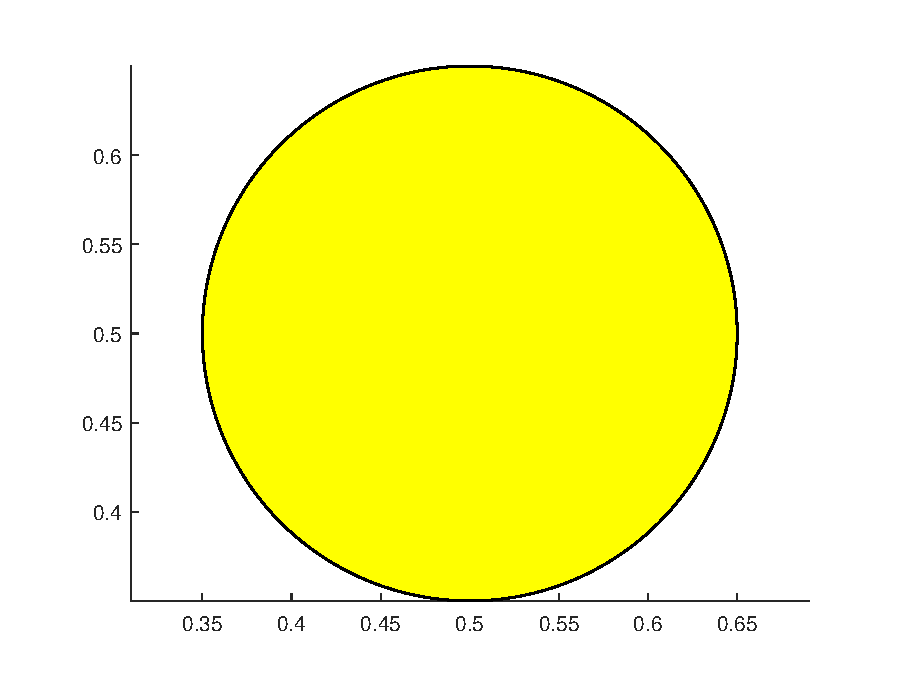
\includegraphics[width=0.3\linewidth]{deformation1T.eps}
    }
    \caption{Deformation: 中间步计算结果图,所用参数为 $n=256$,$k=2\mathrm{e}-2$,$r_\mathrm{tiny}=0.01$。}
    \label{fig:deformation}
\end{figure}

\section{测试结果分析}
从测试结果中可以看到,CPU时间的变化阶数在2左右,除去时间步长每层缩短一半带来的影响,每一步的时间复杂度大约在$\mathrm{O}(n)$,和我们的预期相同。

在CPU时间对比方面,发现\texttt{List}在所有情况下都要比\texttt{Vector}和IMV要慢,因为每一步都创建\texttt{List}临时变量所造成的计算时间增长掩盖了\texttt{List}加减点快带来的计算时间减小。而\texttt{Vector}和IMV相比CPU时间非常接近,IMV相比于\texttt{Vector}优点在于加减点计算量小,缺点在于即使没有进行加减点也要建立临时\texttt{Vector}变量和调用拷贝构造。从测试中我们看到随着示踪点数的增加,IMV的CPU时间有时会低于\texttt{Vector},所以推测随着点数的增加和加减点的更加频繁,IMV相比于\texttt{Vector}应该会有一定优势。

\end{document}